 
 
\chapter{Testing} 
 
 
 
\section{Hvorfor teste} 
 
 
En viktig del av rapporten var å finne ut hvordan animasjoner og lyd påvirker barns opplevelse av programvaren når de bruker en øyesporingsenhet til interaksjon med maskinen. En fremgangsmåte vil være å teste å på et vanlig utvalg mennesker og tolke disse resultatene. Problemet er at resultatene ikke nødvendigvis vil være det samme for barn som med voksne. Som også Nielsen poengterer og tidligere referert at mens barn finner animasjoner og lyder til å være spennende, vil voksne være mindre mottakelige og kan til og med finne dem irriterende. Det ble derfor bestemt at deltakerne måtte nærmest opptil målgruppen for at det skulle være noe poeng med testingen. Så ved å utføre testen var det spesielt to ting vi ønsket å finne ut. Den første var å finne ut om målgruppen greide å bruke prototypen. Vil de greie å navigere og utføre de mest nødvendige oppgavene som å skrive en setning, viske ut ord og gjøre det om til tale. Den neste var som nevnt tidligere å finne ut effekten animasjoner og lyd har når barnet skal bruke programvaren.  
 
 
 
\section{Rekruttering av testere} 
 
 
For å rekruttere deltakere til testen ble først pedagogisk avdeling ved høgskolen i Bergen kontaktet. De hadde tidligere hatt erfaring med å teste på den ønskede målgruppen, og målet var at disse kunne sette oss i kontakt med nøkkelpersoner og i tillegg gi retningslinjer og tips angående det å bruke barn med funksjonshemninger til undersøkelser. Gjennom dette møte ble vi satt i kontakt med Pedagogisk-psykologisk Tjeneste(PPT). PPT er kommunal tjeneste som skal hjelpe barn, ungdom og voksne som strever i utviklingen, eller som har en vanskelig opplæringssituasjon. Blant annet ved å gi systemrettet støtte, med råd og veiledning til skoler om pedagogisk ledelse av gruppe- og læringsmiljø, og bistand med kompetanse- og organisasjonsutvikling \cite{Udir.5:online}. De hadde god erfaring med målgruppen og hadde et større kontaktnettverk enn ved høgskolen. Gjennom PPT ble det sendt ut et informasjonsskriv til foresatte av barn som passet inn i målgruppen hvor det ble gjort rede for hvordan undersøkelsen ville bli gjennomført og hvilke og hvor lenge data ville bli lagret. For at testingen skulle gjennomføres måtte en av barnets foresatte signere og returnere skjemaet. Uheldigvis var det ingen av de foresatte som ønsket at barnet skulle delta i undersøkelsen. Gruppen ble derfor enige om at programvaren uansett måtte testes og at det nærmeste da ville være barn i samme alder som målgruppen, men uten funksjonshemningene. Det ble etter en kontaktrunde klart at 6 foresatte med barn ved Krohnengen barneskole hadde gitt sin tillatelse til å la barna delta i undersøkelsen. 
 
 
\section{Gjennomføring av test} 
 
 
\subsection{Pilottest} 
 
 
Før testingen ble det utført en pilottest på skolen med 4 medstudenter. Dette ble gjort for at testingen skulle gå best mulig og for å identifisere tekniske feil og eventuelle andre hindringer som kunne oppstå underveis.  
 
 
\subsection{Sted} 
Eksperimentet ble utført på Krohengen barneskole inne på biblioteket mellom klokken 13:00 - 
16:00. Dette rommet ble valgt fordi det var nært lokale hvor barna oppholdt seg og fordi det var 
stille. Det var ingen andre barn utenom deltakeren i rommet når testen ble utført. 
(Bilde av testrom og utstyr)  
 
 
\begin{figure}[ht!] 
\centering 
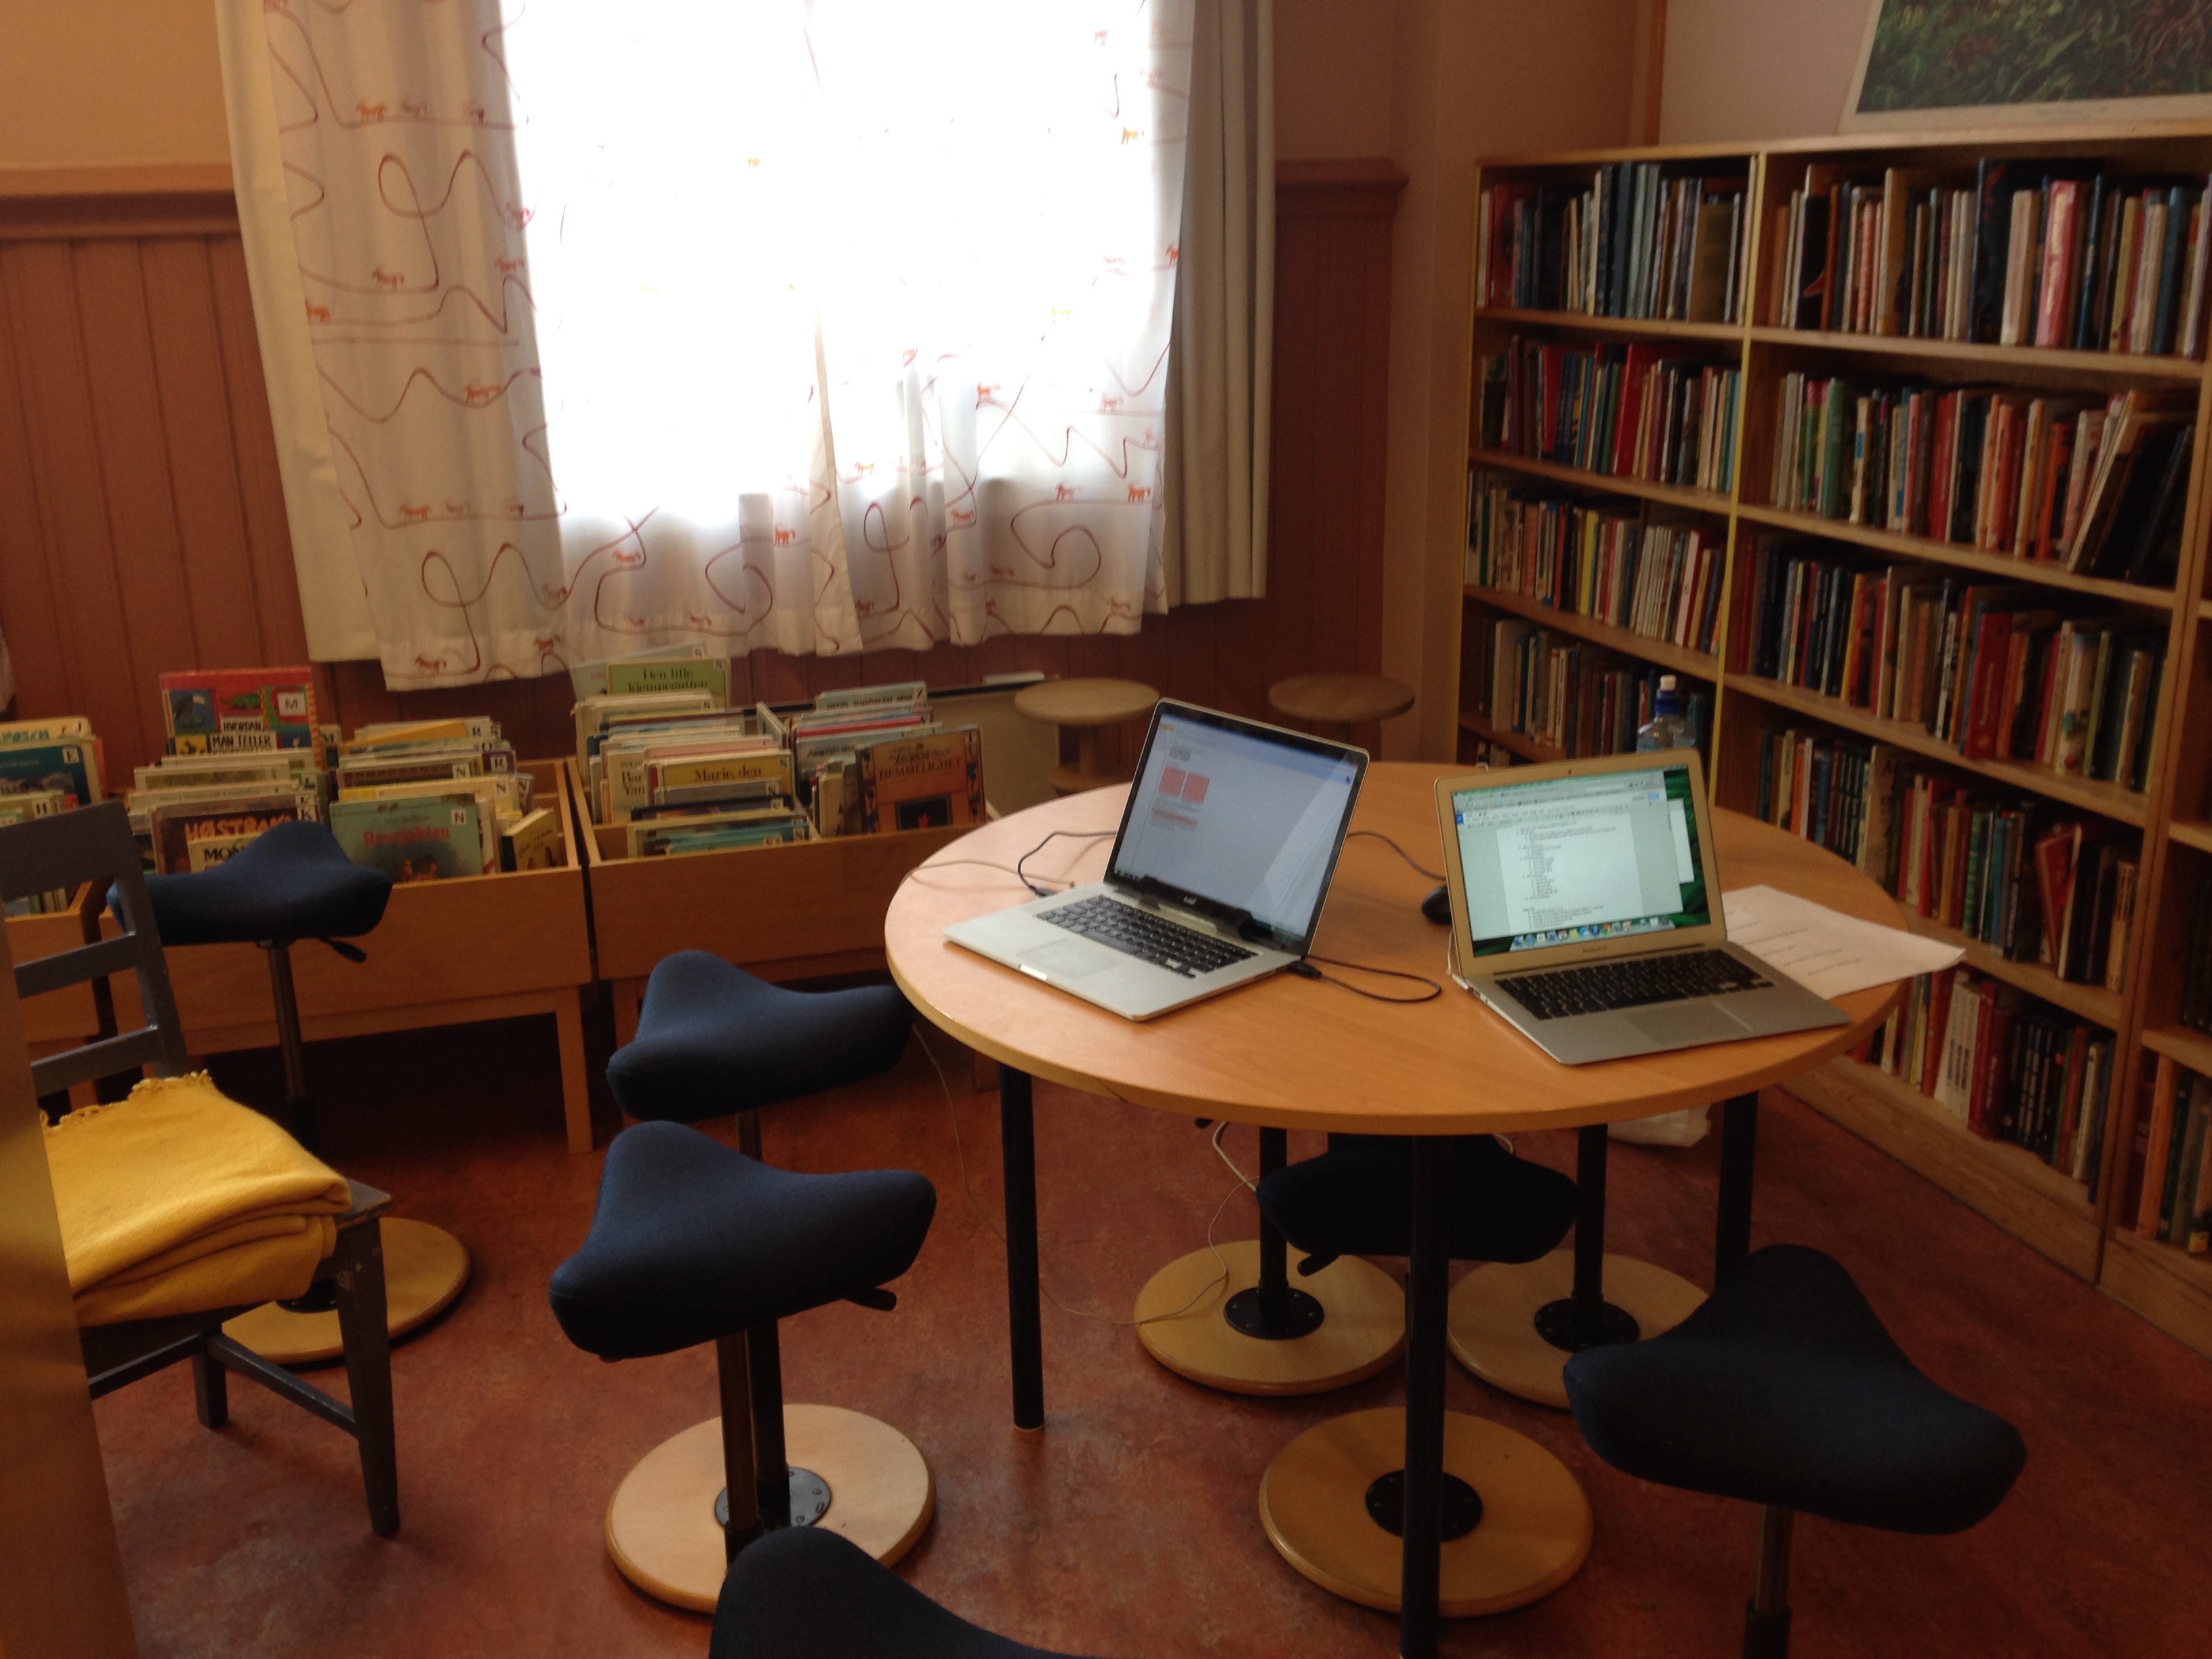
\includegraphics[width=100mm]{Lokale} 
\caption{Bilde av testlokale} 
\label{fig:test_lokale} 
\end{figure} 
 
 
 
 
\subsection{Testgjennomføring} 
Hver test ble gjennomført ved at et og et barn kom inn i biblioteket hvor det først ble foretatt en kort 
samtale for at barnet skulle føle seg komfortabel. Under testingen var kun deltaker og testleder 
tilstedeværende for unngå distraksjoner. Barnet ble så satt foran datamaskinen og øyesporingsenheten satt slik at den siktet på deltakerens ansikt. For at øyesporingsenheten skulle bli mest nøyaktig måtte den tilpasses for hver bruker ved 
en kalibreringsprosess. Prosessen foregikk ved at brukeren følger en rød prikk som starter i 
venstre hjørne og traverserer over skjermen to ganger før den stopper nede i høyre hjørne. Dette 
tar cirka 30 sekund. Etter hver test ble det gitt en farge som beskrev hvor godt enheten greide å 
tilpasse seg brukeren. Rødt er dårligst og programvaren vil ha vanskeligheter med å regne ut hvor 
brukeren ser på skjermen. Gul vil si at kalibreringen gikk greit og at brukeren skal kunne bruke 
enheten på en god måte. Grønn er den mest nøyaktige kalibreringsgraden og enheten vil presist 
fange opp hvor brukeren skuer. Hvis en bruker fikk kalibreringsgrad rød, ble prosessen gjentatt en 
gang. Hvis det igjen viste seg å bli rød ble brukeren bedt om å bruke mus. Kalibreringsgraden ble 
notert for alle brukerne. Deretter ble programvaren startet, og brukeren fikk lov å utprøve programvaren før selve testen startet. 
 
 
Testen startet med at brukeren ble  gitt 5 oppgaver som han skulle gjennomføre. En bruker ble kun presentert for en ny oppgave når den forrige var fullført. Hver oppgave hadde en makstid på 5 minutt. Det vil si at hvis deltakeren brukte mer enn dette ville oppgaven bli registrert som feil og avsluttet. Brukeren ville så bli tildelt neste oppgave. Denne makstiden ble valgt utfra pilottestingen, der brukte deltakerne ca. 30 sekund per oppgave, og med tanke på at disse var i 20 årene ble det også lagt til en god sikkerhetsmargin. Under testingen ble det forsøkt å gi minst mulig spørsmål og ledetråder for å ikke forstyrre eller hjelpe brukeren, ettersom dette ville ha påvirket resultatet. Når brukeren hadde gjennomført alle oppgavene ble han stilt 5 spørsmål. Til slutt ble deltakeren takket for deltakelsen og tildelt et trekk til sykkelsete som kompensasjon. 
 
 
\section{Datainnsamling} 
 
 
For å samle inn data ble det brukt flere ulike metoder.  
 
 
\subsection{Loggfører} 
En viktig del av undersøkelsen var å se hvor lang tid og hvor mange trykk deltakeren brukte på å utføre de forskjellige oppgavene som han ble tildelt. For å gjennomføre dette ble det brukt en logger som lagret data for hver test på separate tekstfiler. Grunnen til at en logger ble brukt er fordi data lagres i et standardformat som gjør at en enkelt kan kjøre spørringer mot det og dermed hente ut målbar data. Data lagres også med en presisjon på tid som en menneskelig observatør ikke har mulighet til og er ikke like mottakelig for feil. Den har også den fordelen at den ligger i bakgrunnen uten brukeren merker noe til den samtidig som den ikke har noen merkbar innflytelse på programvarens ytelse. 
 
 
Så for hver test blir det først logget starttidspunktet, om animasjoner er på eller av, alderen til barnet og om den nødvendige kalibreringen er blitt fullført. Deretter er det kun data fra interaksjoner brukeren gjør med programvaren som blir lagret. Ettersom brukeren kun har mulighet til å trykke på brikker kan det forenkles til at hver gang deltakeren trykket på en brikke ble data logget. Så for vært for vært trykk på en brikke ble det lagret hva som sto på brikken, hvilken type brikken var av og tidspunktet. 
 
 
 
 
\subsection{Skjermopptak} 
 
 
Loggeren fanger kun opp interaksjoner deltakeren gjør med programvaren, noe som utelater det som skjer imellom hver interaksjon. For å kompensere for dette ble det bestemt å ta i bruk en skjermopptaker som kunne fange opp hendelser mellom trykk. Noe som kunne være interessant for å se hvor brukeren nesten trykket og hvordan han beveget blikket, og generelt andre unntak som måtte oppstå. En stor ulempe med skjermopptak er at en observatør fysisk må se igjennom opptaket for å kunne hente ut informasjon, i motsetning til loggeren, hvor store mengder data enkelt kan hentes ut og måles opp mot hverandre. 
 
 
Skjermopptakeren ble som med loggeren startet på nytt for hver test og lagret som separate mp4 filer.  
 
 
 
 
\subsection{Observasjon} 
 
 
Som en del av det å senke terskelen for at foresatte skulle tillate barna å delta i eksperimentet ble det valgt å ikke filme barna under testing. Dette gjorde derimot at en ikke fikk med seg reaksjoner eller spørsmål som ble stilt underveis. Så for å kunne fange opp dette ble det brukt en observatør til å notere ned eventuelle hendelser og spørsmål som deltakeren måtte gjøre seg underveis. Ulempen med dette er at man ikke har samme mulighet som med film til å undersøke det i ettertid. Hvis man går glipp av noe er det ikke mulig å spole tilbake for å se det igjen. Det kan også virke forstyrrende på en deltaker at en person noterer det han foretar seg.  
 
 
 
 
 
 
\subsection{Intervju} 
 
 
Etter at deltakeren har gjennomført oppgavene vil det bli gjort et kort semi-strukturert intervju. Som vil si at spørsmålene er forhåndsdefinerte som i en undersøkelse, men med mulighet for å komme med oppfølgingsspørsmål for å få klarhet i svarene. Intervjuet ble gjort for å undersøke ting som det ikke var mulighet til å fange opp med automatiske verktøy. Blant annet hvordan brukeren opplevde programvaren og hva han syntes om den. 
 
 
 
 
\section{Oppgaver} 
 
 
Som en del av eksperimentet vil deltakerene bli gitt oppgaver som går ut på enten å finne frem enkle ord eller kombinere flere ord til å bygge setninger. For at å kunne gi det beste sammenligningsgrunnlaget vil alle deltakerne bli tildelt de samme oppgavene. 
 
 
Den første oppgaven vil være å finne ordet "hvordan". Denne brikken ligger på første siden og skal være enkel å finne. Meningen med dette er at deltakeren skal forstå hvordan oppgavene er oppbygd og samtidig få litt selvtillit til de neste oppgavene. 
 
 
Den andre oppgaven er litt verre å går ut på at man skal finne brikken hvor det står "banan". For å finne denne må man trykke inn på kategorien "Mat og Drikke" for så å finne brikken med "banan", som i dette tilfelle vil være på den første siden inne på kategorien. Vanskelighetsgraden vil øke en del fra første oppgaven, men antagelsen er at det skal være enkelt å forstå at en må trykke på "mat og drikke" for å finne "banan". Ihvertfall i motsetning til mer abstrakte kategorier som "verb" og "pronomen". 
 
 
Tredje oppgaven er å finne brikken hvor det står "Elg". På samme måte som med "banan" må man også her først finne den passende kategorien. Antagelsen er også her at den skal være rimelig grei å finne for barna med tanke på at den ligger under "dyr". Forskjellen her iforhold til forrige oppgave er at man ikke vil finne brikken på første siden, men må navigere seg over til neste side. 
 
 
I den fjerde oppgaven ønsker vi at deltakeren skal skrive "Jeg vill ha banan", og er med det den første oppgaven hvor deltakeren må kombinere ord for å bygge en setning. Det er derfor valgt en rimelig enkel setning der de to første brikkene "jeg" og "vill ha" er lokalisert på den første siden og det siste ordet har deltakeren funnet en gang før. Dette er gjort for at hinderet fra å finne et ord til flere ikke skal bli for stort.  
 
 
Den femte oppgaven går ut på at deltakeren skrive setningen "Jeg liker katt". Igjen vil de to første ordene være på første siden, mens det nest vil finnes under kategorien "Dyr" som barnet tidligere har vært innom i tredje oppgaven når han skulle finne "Elg".  
 
 
\section{Resultat} 
 
 
\subsection{Observasjon} 
 
 
Hver test startet ved at SFO lederen hentet neste deltaker fra oppholdsrommet og tok dem med til biblioteket hvor undersøkelsen fant sted. De ble så presentert for testlederen av en SFO ansvarlig for at barnet skulle føle seg trygg. Det ble så stilt et par spørsmål, hovedsakelig for å lette på stemningen, men testleder ønsket også å finne ut om noen av barna hadde prøvd øyesporing før, noe ingen av dem hadde. 
 
 
Før selve testen startet, ble testdeltaker satt på stol foran datamaskinen med programvaren og bedt av testleder om å gå kalibrere øyesporingsenheten. Kalibreringen gikk som tidligere nevnt utpå å følge prikken som gikk frem og tilbake over skjermen. Her valgte flere av deltakerne å bevege hodet mer enn øyene, og ble dermed bedt om å prøve å holde hodet stille. Flere reagerte på dette med å stirre intenst på prikken som fløyt over skjermen, noe som gjorde at deltakerne i etterkant fikk litt vondt i hodet. I tre av tilfellene gikk kalibreringen så dårlig at den måtte gjentas. Dette virket negativ inn på barna og ga fra seg lyder med negative assosiasjoner. I et tilfelle ble også den andre runden med kalibrering så dårlig at det ikke ville gitt meningen å bruke øyesporing. Det ble derfor bestemt at deltakeren skulle gjennomføre testen med data mus. Dette ble notert og vil bli tatt hensyn til i evalueringen av data. 
 
 
Når kalibrering var ferdig, ble programmet startet. Her blir deltakeren først presentert for en introduksjonsskjerm og  bedt om å velge sin alder av et utvalg på 3 knapper. Her var det flere som med en gang rakk mot styringsflaten for å trykke på knappen med fingrene, ettersom de ikke var vant til å styre med øyene. Det var derimot det eneste tilfelle hvor testleder måtte gjør deltakerne oppmerksom på at de skulle bruke øyene. 
 
 
Når brukeren var ferdig med introduksjonen starter det som er selve programvaren og som skal testes. Her ble hver deltaker oppfordret til  å prøve å trykke på et par knapper med øyene for å bli kjent med følelsen og hvordan interaksjonen fungerte. Den første oppgaven ble så gitt til deltakerne, finn brikken hvor det står "Hvordan". Det kunne da virke som om flere av deltakerne ble litt stresset. For mens de lette rundt på skjermen etter den korrekte brikken så begynte tiden på hver brikke å gå. Det vil si hjulet som sier hvor lang tid som gjenstår før det blir registrert som et klikk. Dette gjorde at de ble tvunget til å raskt flytte blikket rundt for å unngå trykk på uønskede brikker. Det kan altså se ut som om timeren som begynner når en bruker ser på en brikke tar veldig mye oppmerksomhet vekk fra den faktiske oppgaven. Som er å lete etter rett brikke. Dette gikk igjen under alle oppgavene og gjaldt for alle deltakerne. Dette er nødvendigvis ikke noe som kun gjelder på barn ettersom vi også ble oppmerksom på denne tendensen under pilottesten. Opptil flere ganger gikk tidtakeren helt ut som gjorde at programvaren registrerte det som et trykk og brikken ble flyttet til setningslisten. En deltaker  der animasjoner var slått på, brukte brukeren tid på fjerne feil trykk ved å trykke på slette knappen, mens de andre hele tiden lot feil trykk være. Testleder ga aldri noen hint om at deltakerne trengte å gjøre dette.  
 
 
Andre oppgaven var å finne ordet "banan", noe som økte vanskelighetsgraden et hakk ved at barnet først måtte finne den passende kategorien, før han kunne finne rett brikke. Som med den første oppgaven begynte de å lete etter brikken i leseretning. Testleder spurte deltakerne under denne oppgaven om så på bilde eller leste teksten under for å finne rett brikke. Ingen av deltakerne ble forklart at flere av brikkene var kategorier, noe som gjorde at etter å ha sett over alle brikkene kunne opplyse at de ikke kunne finne brikken hvor det sto "banan". 
Det ble da gitt et tips fra testleder om at noen brikker kunne gjøre slik at det dukket opp flere og at de måtte finne den. Når den var sagt var det ingen som brukte lang tid på finne fram til den korrekte kategorien og deretter finne banan brikken.  
 
 
Etter å ha skrevet banan ble de bedt om å finne brikken hvor det sto elg. Deltakerne så da ut til å automatisk lete blant kategori brikkene og tiden brukt på å finne rett kategori var kort. Problemet her var at brikken hvor det sto elg, befant seg ikke på den første siden, men andre. Så får komme til denne må en navigere seg til neste side. Her varierte det svært mellom deltakerne. En så blant over alle brikkene og når han ikke fant den ønskede så var han på vei til å navigere seg tilbake istedenfor til neste side. En annen deltaker hadde derimot mer korrekt fremgangsmåte. For etter raskt å ha konstatert at brikken ikke fantes på den aktuelle siden, så trykket han til neste side og fant brikken.  
 
 
 
 
Med de tre første oppgavene unnagjort skulle deltakerne kombinere det de hadde lært ved å skrive den enkle setningen "jeg vil ha banan". Ingen av barna hadde noe særlig problem med å finne de to første ordene,  og det tredje hadde alle allerede funnet en gang, men allikevel var det to som ikke automatisk kom på dette og igjen begynte å se over kategoriene. Alle så ut til å håndtere overgangen fra enkle ord til setninger svært bra. Slik at når de kom på tredje oppgaven som var å skrive "Jeg liker katt" så begynte med en gang uten noen videre beskjeder fra testleder. Til tross for at de ikke hatt brukt brikken "katt" før, så fant de raskt frem rett kategori. Det som skjedde så var litt mer oppmerksomhetsvekkende. For inne på første siden finnes det i tillegg til brikken hvor det står "katt" også en brikke hvor det står "kattunge". Det som skjedde var at samtlige av testdeltakerne valgte sistnevnte. Å på spørsmål fra testleder om hvorfor de gjorde dette, så var det en så svarte at oppgaven var å finne "katt". Deltakerne ble derfor spurt spørsmål om de baserte brikketrykkene sine på teksten eller bildet. Hvor samtlige av barna svarte at bildet. Noen som ikke bare forklarte hvorfor de valgte "kattunge", men også hvorfor det virket lettere for deltakerne å finne kategorien "dyr" over "mat og drikke". For mens "dyr" var representer med ulike dyr, så var "mat og drikke kun representert av drikkevarer. Noe vi ble oppmerksom på i etterkant. 
 
 
 
 
Til tross for at ingen av deltakerne hadde brukt øyesporing før, fikk alle det til. Utenom deltakeren der kalibrering ikke helt fungerte. Ingen feil dukket opp, og alle deltakerne greide å gjennomføre oppgavene. Selv om det var relativt få oppgaver greide de dem uten noe særlig behov for å tenke seg om. Utfra observasjonene kan en slå fast at for en førstegangsbruker så kan tidtakeren som vises gå litt i raskeste laget og en bør muligens se på alternative måter å vise denne. Ettersom det skjedde flere feiltrykk og deltakerne ble stresset og visste ikke hvor de skulle hvile blikket mens de lette. Det kan også slå fast at de i hovedsak bruker bildet til å finne rett brikke noe som gjør at bildet bør vise klart hva det representerer og unngå tvetydighet.  
 
 
 
 
\subsection{Intervju} 
 
 
Med det semi-strukturerte intervjuet ønsket vi å finne ut hvordan barna opplevde å bruke prototypen. Problemet var at uansett hvordan spørsmålet ble formulert var deltakerne utelukkende positive. Eksempelvis så ga alle karakteren 10 på en skala fra 1 til 10, og på oppfølgende spørsmål om det var ingenting som burde vært annerledes, så var svaret nei. Dette gjorde at flere av spørsmålene som ble stilt ble forkastet.  
 
 
Et spørsmål som var interessant var når testleder pekte på det 
 
 
Det semi-strukturerte intervjuet startet rett etter at en deltaker var ferdig med å utføre oppgavene på prototypen og tok relativt liten tid. Grunnen til dette  
En tendens som testleder var klar over på forhånd er at barn er utelukkende positive og vil sliter med å gi gjennomtenkte svar. Flere av barna i dette eksperimentet var også sjenerte, noe som gjorde at det en måtte presse litt for å få et form for svar.  
 
 
\subsection{Tid} 
 
 
En ting som vi ønsket å finne ut var hvorvidt animasjoner gjorde at deltakerne brukte lengre tid per oppgave eller ikke. For å finne ut dette ble tiden hver deltaker brukte per oppgave registrert.  
 
 
\begin{figure}[ht!] 
\centering 
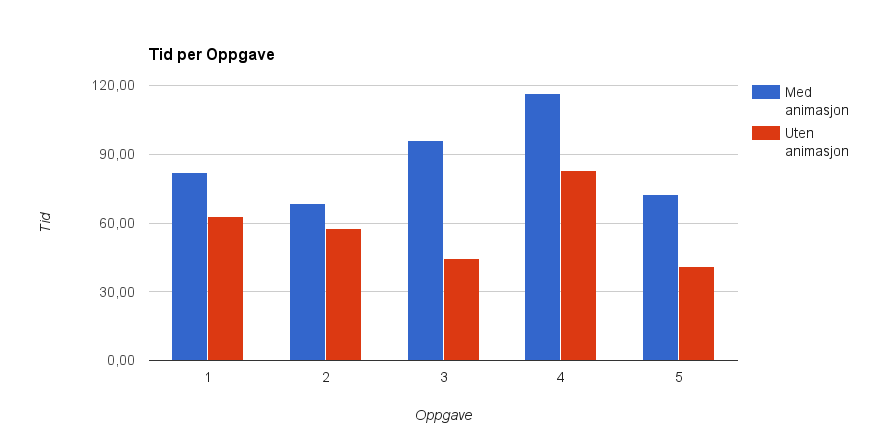
\includegraphics[width=100mm]{TidPerOppgave} 
\caption{Diagram som viser gjennomsnittlig tid per oppgave delt inn i to grupper basert på om animasjoner var på eller ikke.} 
\label{fig:DiagramTidPerOppgave} 
\end{figure} 
 
 
I Diagrammet \ref{fig:DiagramTidPerOppgave} viser den blå søylen den gjennomsnittlige tiden det tok for deltakerne som hadde på animasjoner å gjennomføre oppgaven, mens den røde viser hvor lang tid det tok for de uten. Som man kan se utifra denne så ser man at tendensen er at de som hadde på animasjoner brukte lengre tid en de uten. Noe som kan tyde på at animasjoner gjør at en bruker lengre tid ved å ha animasjonene slått på.  
 
 
 
 
 
 
 
 
 
 
 
 
 
 
 
 
 
 
\section{Tolkning av resultat} 
 
 
Det er viktig å poengtere at testen kun hadde 6 deltakere og at det derfor ikke vil bli forsøkt å gitt noe form for bevis på at disse resultatene vil kunne reproduseres. Dataene vil i beste fall kun gi indikasjoner.  Med testingen ønsket vi å undersøke hvorvidt målgruppen greide å utføre de mest nødvendige oppgavene i prototypen og hvilken påvirkning animasjoner og lyd hadde på barnet.  
 
Deltakerne hadde ingen erfaring med bruk av øyesporingsenheten eller lignende programvare. Allikevel tok det ikke lang tid før de tilpasset seg og trykket på de forskjellige symbolene. De hadde ingen spørsmål rundt hva som regnet som et klikk eller hva de ulike menyknappene betydde. Deltakerne greide også å gjennomføre alle oppgavene de ble tildelt. En liten oppdagelse ble derimot gjort, alle deltakerne hadde problemer med at nedtellingsklokken, som viser på symbolet hvor lenge det er igjen til det blir regnet som et trykk, gikk altfor fort. Dette var også en erfaring som ble gjort under testingen på medstudenter.  Det var derimot ikke nok til å hindre deltakerne i å operere programvaren og gjennomføre alle oppgavene. Spørsmålet blir da hvorvidt man kan si om barn i målgruppen kunne utført de mest nødvendige operasjonene på prototypen, med tanke på at deltakerne som ble testet var barn, men uten noen form for funksjonshemning. Forskjellen er at målgruppen har en funksjonshemning. Selv om vi hadde fått testet på målgruppen hadde dette vært en usikkerhetsfaktor, ettersom det finnes flere funksjonshemninger og flere grader av dem. Slik at det man kan si utfra testingen er barn i 6 års alderen har ingen store problemer med å skrive og finne frem til de korrekte ordene og man kan derfor fastslå at et barn i målgruppen også vil hatt mulighet om ikke like lett kunne uttrykke seg selv gjennom prototypen. 
 
I tillegg vil testen også finne ut hvilken effekt animasjoner og lyd ville ha. For å finne ut dette ble data samlet mens deltakerne utførte 6 oppgaver som ble tildelt. Dataene er presentert i diagram og gir klare indikasjoner på at deltakerne som hadde animasjoner og lyd brukte lengre tid på oppgavene enn de uten. Dette er interessant, men det skal igjen nevnes at i tillegg til at det var kun 6 deltakere var det også kun 6 oppgaver som de gjennomførte. Til tross for at de brukte lengre tid på å gjennomføre oppgavene, var det kun de 2 av 3 som hadde animasjoner på som kunne svare hva som skjedde ved å trykke på en kategori- og ordsymbol. Hvis dette skulle stemme så kan det tyde på at en bruker kanskje burde starte med å ha animasjoner på for så etter en stund skru dette av.  
 
 
Som en oppsummering så kan en si at med så lite testpersoner så kan man ikke si noe sikkert, men vi kan konkludere med at prototypen fungerer og at et barn i seks år alderen enkelt greier å uttrykke seg via denne. I tillegg er det indikasjoner på at animasjoner gjør at en ny bruker av programvaren bruker lengre tid enn uten animasjoner. Det er også indikasjoner på animasjoner og lyd gir brukeren en bedre forståelse for hva de ulike typene symbol representerer.  
 
 
 
 
 
 
// Som sagt kun indikasjoner, men spennende og trenger mer forskning og testing 
// Vanskelig å si noe 
//Resultatene viser indikasjoner på at de bruker lengre tid med animasjonr, men også indikasjoner på at de forstår det bedre. Litt uforståelig. De andre greide også komme inn på kategorien. Kan være at de bare ikke forsto spørsmålet eller noe i den duren. 
//dette satt sammen med at de kan 
 
 
 
 
//barn og har ikke prøvd øyesporing før 
//Selve øyesporing fungerer på samme måte som i sono flex. Ihvertfall besvist at den fungerer 
 
 
 
 
 
 
//Disse var som sagt ikke innen for målgruppen 
 
 
som alle slet med, til og med meds 
 
 
 
 
Til tross for dette greide alle å fullføre oppgavene de ble Allikevel gjennomførte alle oppgaven 
 
 
 
 
 
 
 
 
 
 
//uten noe form for opplæring greide de å skrive fullstendige setninger 
// Hadde noen problemer med at nedtelling for klikk gikk for fort 
//ingen problemer som også ikke eksisterer i Sono Flex 
 
 
 
 
2. 
 
 
 
 
 
 
 
 
 
 
 
 
http://www.udir.no/Regelverk/tidlig-innsats/Skole/Oversikt-over-aktorene/PP-tjenesten/  
 